\documentclass[12pt]{beamer}
\usetheme{Madrid}

\usepackage{amsmath, amsfonts}
\usepackage{hyperref}
\usepackage[super,comma,numbers]{natbib}
\renewcommand{\bibnumfmt}[1]{[#1]}
\bibliographystyle{apsrev4-1}

\title{Diffusion through semi-permeable membranes}
\author[A. Brown]{Aiyan B.}
\date{November 26, 2025}

\newcommand{\abs}[1]{\left| #1 \right|} % | |

\begin{document}

\maketitle

\begin{frame}{A finer picture of the fence model}
    \begin{itemize}
        \item The fence model~\cite{Kusumi2005} proposes that the membrane-skeleton (MS) forms ``fences'' which restrict the motion of transmembrane proteins (TMP) through the plasma membrane (PM)
    \end{itemize}
    \begin{figure}
        \centering
        \includegraphics[width=0.8\textwidth]{figures/hop-diffusion.jpg}
    \end{figure}
    \pause
    \begin{itemize}
        \item There is no currently microscopic model for how this hop-diffusion occurs: can we build one?
    \end{itemize}
\end{frame}

\begin{frame}{Shortcomings of current models}
    \begin{columns}
        \begin{column}{0.35\textwidth}
            \begin{itemize}
                \item MS is a rather non-trivial structure, far from this naive square fence perspective
                \pause
                \item No clear picture as to why long-time high-density regions/ ``hot-spots'' exist
            \end{itemize}
        \end{column}
        \pause
        \begin{column}{0.65\textwidth}
            \begin{figure}
                \centering
                \includegraphics[width=0.55\textwidth]{figures/mem-skel.jpg}
                \caption{Taken from Morone et al. (2006)~\cite{Morone2006}}
            \end{figure}
        \end{column}
    \end{columns}
\end{frame}

\begin{frame}{Diffusion through a semi-permeable membrane}
    \begin{itemize}
        \item Consider a particle diffusing on a loop $\mathbb{R} \bmod{2 \pi}$
        \pause
        \item At some point, there is a highly localized directional and semi-permeable membrane which alters the diffusive nature.
        In particular, allow crossing from the left with probability $0 \leq \lambda \leq 1$ and from the right with probability $ 0 \leq \kappa \leq 1$
    \end{itemize}
    \begin{figure}
        \centering
        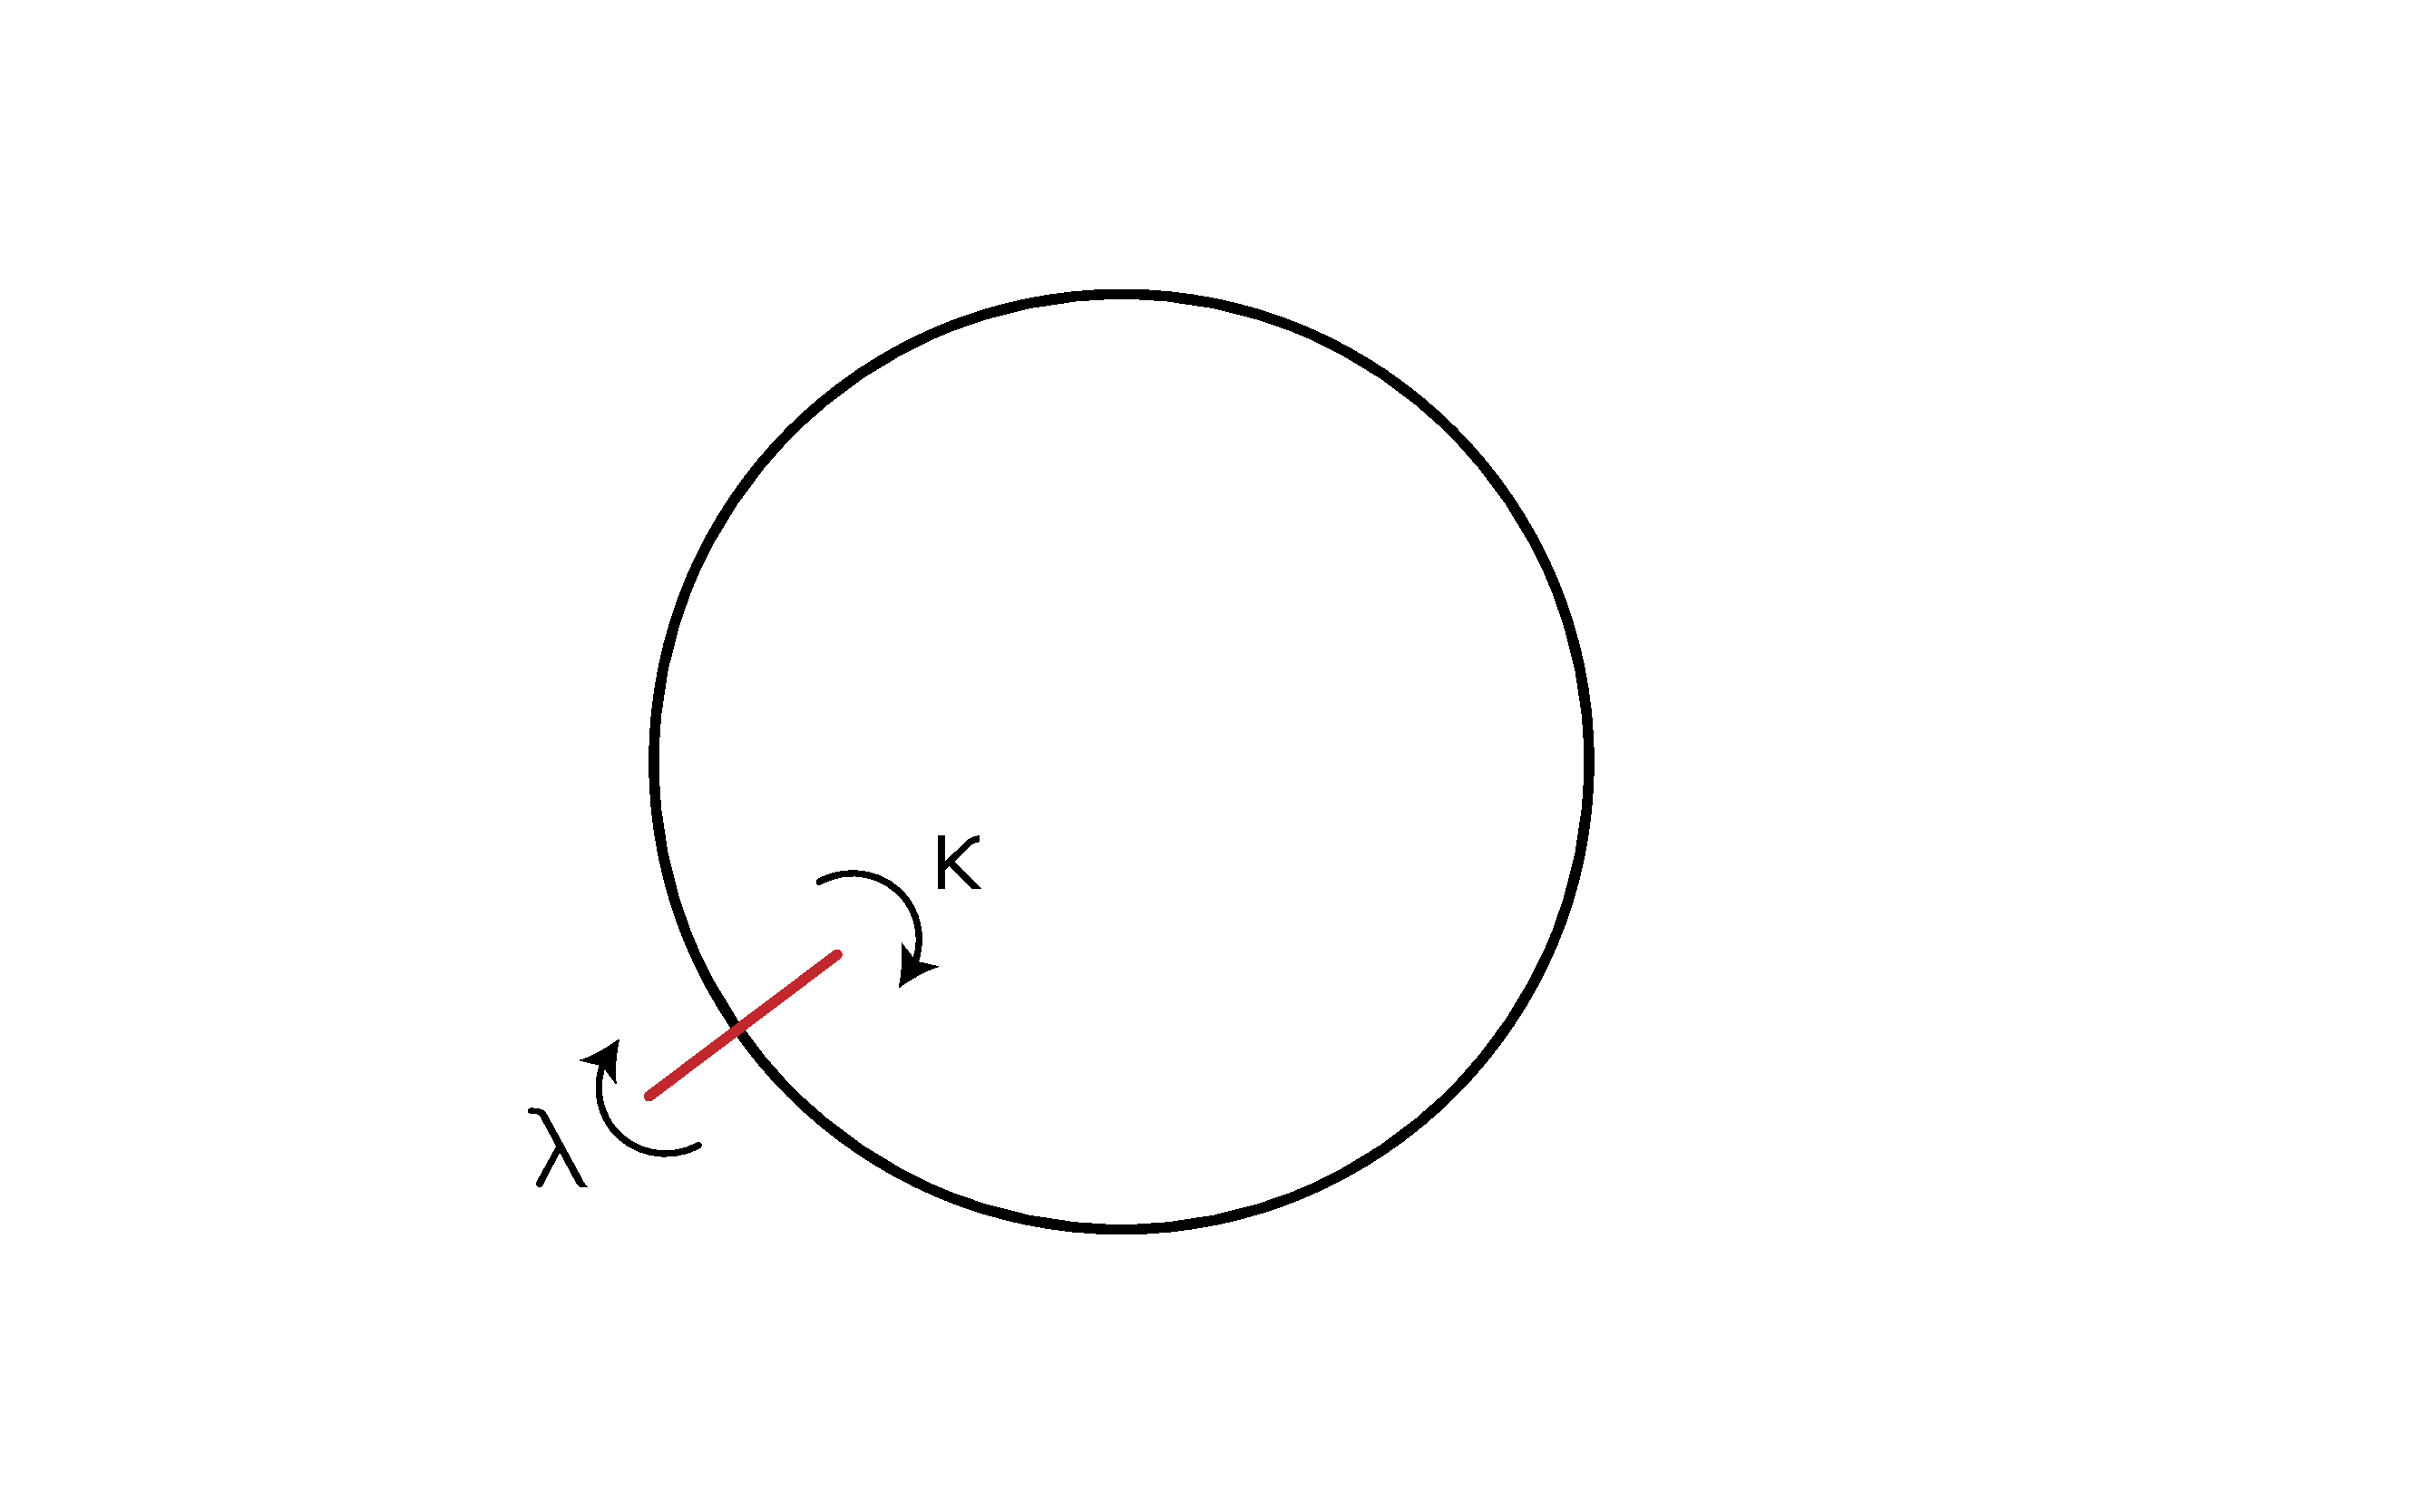
\includegraphics[width=0.45\textwidth]{figures/symmetry-breaking-diff.pdf}
    \end{figure}
\end{frame}

\begin{frame}{The master equation}
    \begin{itemize}
        \item Suppose the membrane occurs at $M \equiv M \bmod{N}$, where there are $N$ elements on the lattice.
        The (discrete) master equation for the system reads
        \begin{multline*}
            \frac{\partial p_j (t)}{\partial t} = \frac{1}{\tau} \left[ \frac{1}{2} p_{j+1} (t) + \frac{1}{2} p_{j-1} (t) - p_j (t) \right] \\
            + \frac{\Delta_\lambda}{\tau} p_M (t) \left( \delta_{M-1,j} - \delta_{M+1,j} \right) + \frac{\Delta_\kappa}{\tau} p_{M+1} (t) \left( \delta_{M+2,j} - \delta_{M,j} \right),
        \end{multline*}
        where $\Delta_s = \frac{1}{2} - s$ with temporal step size $\tau$
        \begin{itemize}
            \item If $\lambda = \kappa = 1/2$, $\Delta_\lambda = \Delta_\kappa = 0$ and we recover the random walk
        \end{itemize}
    \end{itemize}
\end{frame}

\begin{frame}{The continuum equation of motion I}
    \begin{itemize}
        \item Allow $x_j = j a_0$ for lattice spacing $a_0$ and take the limit $\tau, a_0 \to 0$
        \item Dividing the first term by $a_0^2$ and letting $D = a_0^2 / 2 \tau$ remain fixed in the limit, we find
        \begin{equation} \label{eq:1}
            \frac{\partial p (x,t)}{\partial t} = \mathcal{L} (x; x_b) p(x,t),
        \end{equation}
        where the generator, to linear order in $a_0$ is
        \begin{equation} \label{eq:2}
            \mathcal{L} (x; x_b) = D \frac{\partial^2}{\partial x^2} + 4 D \delta'(x - x_b) \left( \kappa - \lambda - \Delta_\kappa a_0 \left. \frac{\partial}{\partial x} \right\vert_{x = x_b} \right)
        \end{equation}
        \pause
        \begin{itemize}
            \item This is a generalization for $\lambda \neq \kappa$ of the continuum limit presented in Kay, T. \& Giuggioli, L. (2022)~\cite{Kay2022}
        \end{itemize}
    \end{itemize}
\end{frame}

\begin{frame}{The continuum equation of motion II}
    \begin{itemize}
        \item Define $J (x,t) = - D \partial_x p(x,t)$ as the probability current and let $\Delta_\kappa a_0 / \tau \to k$ such that the action of the generator is
        \begin{equation} \label{eq:3}
            D \frac{\partial^2 p}{\partial x^2} + 4 D \left( \kappa - \lambda \right) \delta'(x - x_b) p + \frac{4 \Delta_\kappa^2 D}{k} J(x, t) \delta'(x - x_b)
        \end{equation}
        \pause
        \item We can interpret these terms as follows -- using that the derivative of the Dirac delta acts as $\delta'[\psi] = - \psi' (0)$ --
        \begin{enumerate}
            \item regular diffusion generator;
            \item local drift due to the directional motion at the barrier;
            \item local drift due to flux generation at barrier
        \end{enumerate}
    \end{itemize}
\end{frame}

\begin{frame}{Generalizations}
    \begin{itemize}
        \item The generalization to $d$ spatial dimensions is trivial: 
        define a surface $\Gamma \subset \mathbb{R}^d$ along which there is a barrier and modify $\partial_x^2 \to \nabla^2$ such that, for $t \to \tau = D t$,
        \begin{equation} \label{eq:4}
            (\mathcal{L} p) (\mathbf{x}; \mathbf{x}_b) = \nabla^2 p + \delta'(\mathbf{x} - \Gamma) \left[ a p + b J(\mathbf{x}, \tau) \right] = \mathcal{L}_0 p + \mathcal{L}'p,
        \end{equation}
        where I have defined $a = 4 (\kappa - \lambda)$ and $b = \frac{4 \Delta_\kappa^2}{k}$
        \pause
        \item Also straightforward to generalize Eq.~\eqref{eq:4} to multiple surfaces/ points by performing a sum over all individual surfaces,
        \begin{equation} \label{eq:8}
            (\mathcal{L} p) (x; x_b) = \mathcal{L}_0 + \sum_i \delta'(\mathbf{x} - \Gamma_i) \left[ a p + b J(x, \tau) \right],
        \end{equation}
        where $\Gamma_i$ is the $i$th semi-permeable barrier
    \end{itemize}
\end{frame}

\begin{frame}{A note on a potential path forward}
    \begin{itemize}
        \item Apparent ``random'' structure of the skeleton suggests it  might be useful to define surfaces as the edges of random tessellations
    \end{itemize}
    \begin{figure}
        \centering
        \includegraphics[width=0.7\textwidth]{figures/tessellation.png}
    \end{figure}
\end{frame}

\begin{frame}{A Green's function solution I}
    \begin{itemize}
        \item The non-interacting Green's function solves the problem $(\partial_t - \mathcal{L}_0) G^{(0)} = \delta (\mathbf{x},\tau)$ and is clearly the heat kernel,
        \begin{equation} \label{eq:5}
            G^{(0)} (\mathbf{x}, \tau | \mathbf{x}') = \frac{1}{(4 \pi \tau)^{d/2}} \Theta (\tau) \exp{\left( - \frac{\abs{\mathbf{x} - \mathbf{x}'}^2}{4 \tau} \right)}
        \end{equation}
        or, more simply, in energy-momentum space,
        \begin{equation} \label{eq:6}
            G^{(0)} (\mathbf{k}, \omega) = (i \omega - k^2)^{-1}
        \end{equation}
    \end{itemize}
\end{frame}

\begin{frame}{A Green's function solution II}
    \begin{itemize}
        \item To second order in the Dyson series, $\hat{G} = \hat{G}^{(0)} + \hat{G}^{(0)} \hat{\mathcal{L}}' \hat{G}^{(0)}$.
        We can evaluate this explicitly by understanding the interaction propagator as acting on $G^{(0)}$.
        Returning to one dimension for simplicity,
        \begin{equation} \label{eq:7}
            \frac{G^{(1)} (x, \tau | x')}{G^{(0)} (x, \tau | x')} = 1 + a \frac{x_b - x'}{2 \tau} + b \left( \frac{1}{2 \tau} - \frac{(x_b - x')^2}{4 \tau^2} \right)
        \end{equation}
        \pause
        \begin{itemize}
            \item As $\tau \to \infty$, we approach the same steady state as in the regular heat equation (cannot be the reason for confinement)
            \item As $\tau \to 0^+$, observe convergence in $G^{(1)} (x, \tau | x')$ to zero
            \item At short times, $\tau \sim 0$, increasingly large contributions from higher-order factors to compensate for starting near $x_b'$
            \item When $\lambda = \kappa$, $a = 0$
        \end{itemize}
    \end{itemize}
\end{frame}

\begin{frame}{References}
    \bibliography{references}
\end{frame}

\begin{frame}{Continuum limit I (details)}
    \begin{itemize}
        \item Formally, the discrete-to-continuum mapping is given by the following relationship $\sum_i \to \frac{1}{a_0} \int dx$
        \item Hence $\delta_{M,j} \to a_0 \delta (x - x_b)$ where $x_b$ is the location of the barrier
        \item To this end, the first difference of deltas can be written
        \begin{equation}
            \delta_{M-1,j} - \delta_{M+1,j} \to a_0 \left[ \delta (x - (x_b - a_0)) - \delta (x - (x_b + a_0)) \right]
        \end{equation}
        \item Taylor expanding in the delta functions,
        \begin{equation}
            \delta (x - (x_b \pm a_0)) = \delta (x - x_b) \mp a_0 \delta'(x - x_b) + \mathcal{O} (a_0^3)
        \end{equation}
        and substituting into the Kronecker delta mapping,
        \begin{align}
            \delta_{M-1,j} - \delta_{M+1,j} \to 2 a_0^2 \delta'(x - x_b) + \mathcal{O} (a_0^4)
        \end{align}
    \end{itemize}
\end{frame}

\begin{frame}{Continuum limit II (details)}
    \begin{itemize}
        \item In a similar manner, the second difference of delta functions can be mapped
        \begin{equation}
            \delta_{M+2,j} - \delta_{M,j} \to a_0 \left[ \delta (x - (x_b + 2a_0)) - \delta (x - x_b) \right]
        \end{equation}
        and so, following a series expansion,
        \begin{equation}
            \delta_{M+2,j} - \delta_{M,j} \to - 2 a_0^2 \delta' (x - x_b) + \mathcal{O} (a_0^4)
        \end{equation}
        \item We now return to the inhomogeneous term and note that $p_{M+1} (t) = p (x_b + a_0, t) = p(x_b, t) + a_0 \left. \frac{d p}{dx} \right|_{x = x_b} + \mathcal{O} (a_0^2)$.
        So, to first order in $a_0$,
        \begin{equation}
            \frac{2 \Delta_\lambda a_0^2}{\tau} p (x_b, t) \delta' (x - x_b) - \frac{2 \Delta_\kappa a_0^2}{\tau} \delta' (x - x_b) \left( p(x_b, t) + a_0 \left. \frac{d p}{dx} \right|_{x = x_b} \right)
        \end{equation}
    \end{itemize}
\end{frame}

\begin{frame}{Continuum limit III (details)}
    \begin{itemize}
        \item Reorganizing and using the definitions $\Delta_s = \frac{1}{2} - s$ and $D = a_0^2 / 2 \tau$,
        \begin{equation}
            4 D \left( \kappa - \lambda \right) p (x, t) \delta' (x - x_b) + 4 \Delta_\kappa a_0 \delta' (x - x_b) J(x,t)
        \end{equation}
        \item We now suppose that $\Delta_\kappa a_0 / \tau \to k$ and remains finite in the limit such that
        \begin{equation}
            4 D \left( \kappa - \lambda \right) p (x, t) \delta' (x - x_b) + \frac{4 D \Delta_\kappa^2}{k} \delta' (x - x_b) J(x,t)
        \end{equation}
    \end{itemize}
\end{frame}

\begin{frame}{Energy-momentum space}
    \begin{itemize}
        \item It is convenient to define the Fourier transform as
        \begin{equation}
            G (\mathbf{x}, t) = \int \frac{d^d k}{(2 \pi)^d} \frac{d \omega}{2 \pi} \, e^{i \mathbf{k} \cdot \mathbf{x} - i \omega t} G (\mathbf{k}, \omega)
        \end{equation}
        such that we get a pole in the upper half of the plane
    \end{itemize}
\end{frame}

\end{document}